% ==============================================
% CFD Tutorial Template: OpenFOAM Terminal Basics
% Class: scrartcl (KOMA-Script) - optimized for tutorials
% Content: pitzDaily with simpleFoam
% ==============================================

\documentclass[
    parskip=half,      % Space between paragraphs (better for steps)
    DIV=12,            % Optimal margins for readability
    headings=normal,   % Professional heading sizes
    fontsize=11pt,     % Slightly larger for screen reading
    english            % Language setting
]{scrartcl}

\input{../preamble.tex}

% ========== DOCUMENT START ==========
\begin{document}

% ========== TITLE PAGE ==========
\title{Tutorial \#3: Compressible air Ejector}
\subtitle{Supersonic Transient and Steady Flow}
\subject{Workshop on Computational Fluid Dynamics (CFD) \\ with OpenFOAM \\ IMP-PAN Gda\'nsk}
\author{Robert Castilla \\ CATMech - Universitat Politècnica de Catalunya \\ Department of Fluid Mechanics}
\date{2025-26 \\ Version 1.0}



\maketitle

% ========== ABSTRACT ==========
\begin{abstract}

\end{abstract}

\tableofcontents
\newpage

\fbox{
	\parbox{15cm}{

\section*{Learning Objectives}
By the end of this tutorial the student will be able to
	
	\begin{enumerate}
		\item \textbf{Navigate} OpenFOAM case directory structure
		
		\item \textbf{Understand} basic OpenFOAM file formats
		
		\item \textbf{Run} a simple transient simulation
		
		\item \textbf{Analyze} basic results in terminal and \terminalcmd{paraview}
	\end{enumerate}
}
}
% ========== SECTION 1: INTRODUCTION ==========
\section{Introduction and Theoretical Background}

In this session a supersonic air ejector is simulated. In this case high velocity air is used 
 to create a very low pressure region with a shock wave. after this first shock wave secondary
 flow air is suctioned and mixed with the main jet. This mixed flow is  accelerated in the mixing
 chamber until a second second wave is created is the diffuser. 
 
 This simulation is challenging because of the high Ma number compressible flow. For the 
 previous sessions, where fluid were either liquids of low velocity gas, the simulations
 where performed by using a \textbf{pressure-based solver} (SIMPLE, PISO or PIMPLE algorithm). 
 Momentum balance is computed by defining an equation for pressure (Poisson equation) that
 is corrected with continuity and then again computed with momentum equation until convergence.
 This method is not valid for high Ma number flows, since is not capable to adequately resolve
 shock waves. Instead, a \textbf{density-based solver} is used. These solvers consider energy equation,
 computing pressure from density and perfect gas equation (or any other gas state equation).
 
 Two different approaches for density-based solvers will be considered:
 \begin{itemize}
 	\item  \terminalcmd{rhoCentralFoam} is a transient \textbf{explicit} density-based solver.
 	\item  \terminalcmd{HiSA} is a steady \textbf{implicit} density-based solver.\footnote{It can also be
 	configured to simulate a trasnient flow, but in this session only the steady state case is treated.}
 \end{itemize}
  
 The implicit approach is more stable and robust, but, on the other hand, it requires a 
 more complex solver configuration and is more computational resources demanding, both in time and memory. 

\subsection{Case Overview}

The scheme of the ejector is depicted in Figure \ref{fig:scheme}. Note that the primary nozzle has now the typical convergence-divergent shape in order to speed up the primary flow
and get a shock wave. Also, the outlet has been enlarged in order to avoid as much as possible
pressure wave reflections.

 
\begin{figure}[H]
	\centering
	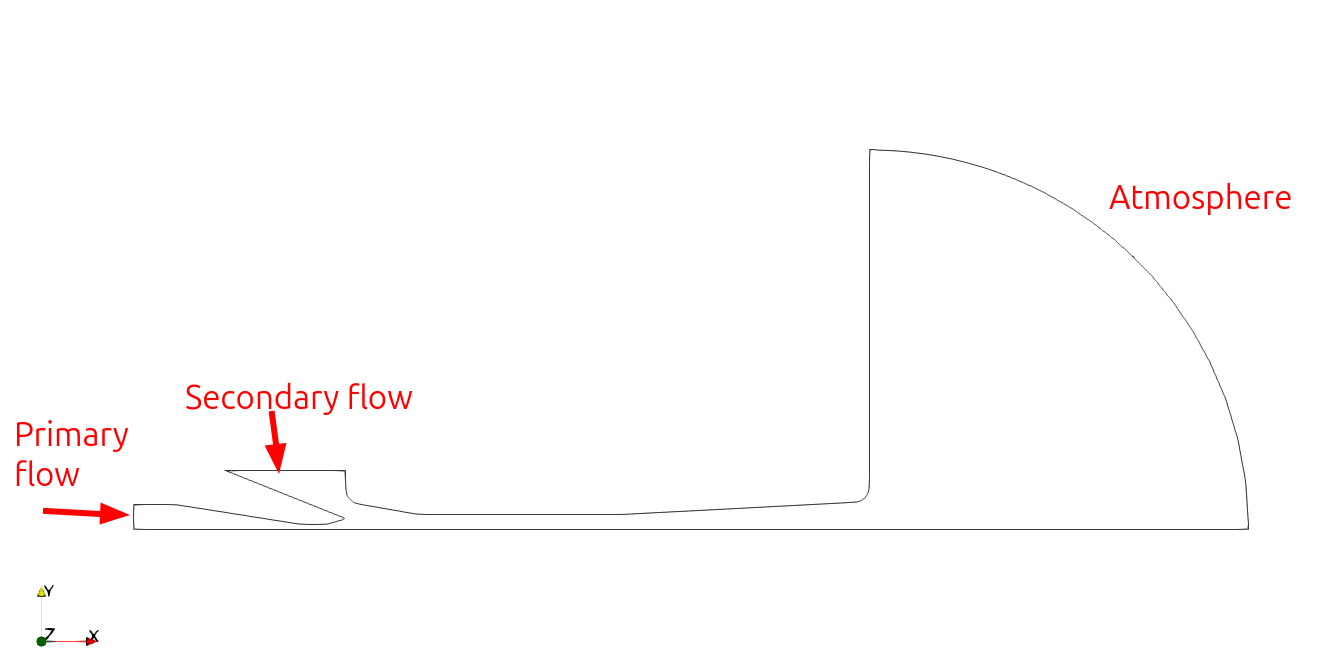
\includegraphics[width=\linewidth]{Figures/Scheme}
	\caption{Scheme of supersonic ejector}
	\label{fig:scheme}
\end{figure}


% ========== SECTION 2: TERMINAL SETUP ==========
\section{Case Setup}

The python environment used in Session 2 has to be also activated for the present tutorial. 



\section{Part A: Density based explicit solver \terminalcmd{rhoCentralFoam}} 

The clean case can be downloaded from the GitHub repository

\subsection{Running the Simulation}

Again, the simulation is split in two parts: the generation of the mesh and running the solver.

\subsubsection{Mesh generation}

To generate the \filename{blockMeshDict} file, run 

Check that the python virtual environment is activated and run
\begin{lstlisting}[style=terminal]
python supersonic_blockMeshDictGen.py
\end{lstlisting}
The \filename{blockMeshDict} is created in the same folder. Move to the \filename{system} folder
of the case to be simulated (now the \filename{rCF} case).

The \filename{genMesh.scr} script runs the \terminalcmd{blockMesh},\terminalcmd{extrudeMesh} and
\terminalcmd{checkMesh} commands.


\subsubsection{Initialization and solver execution}

To run the solver, type

\begin{lstlisting}[style=terminal]
./runCase.scr
\end{lstlisting}

This simulation is very slow. It takes about 4 to 5 hours to run \qty{5}{ms}. But this is enough
to get a steady state flow. Hoew



\subsection{Post-Processing in Terminal}


\subsection{Visualization in paraview}



\section{Part B: Density based implicit solver \terminalcmd{HiSA}}


\subsection{Post-Processing in Terminal}


\subsection{Visualization with paraview}

\begin{figure}[H]
	\centering
	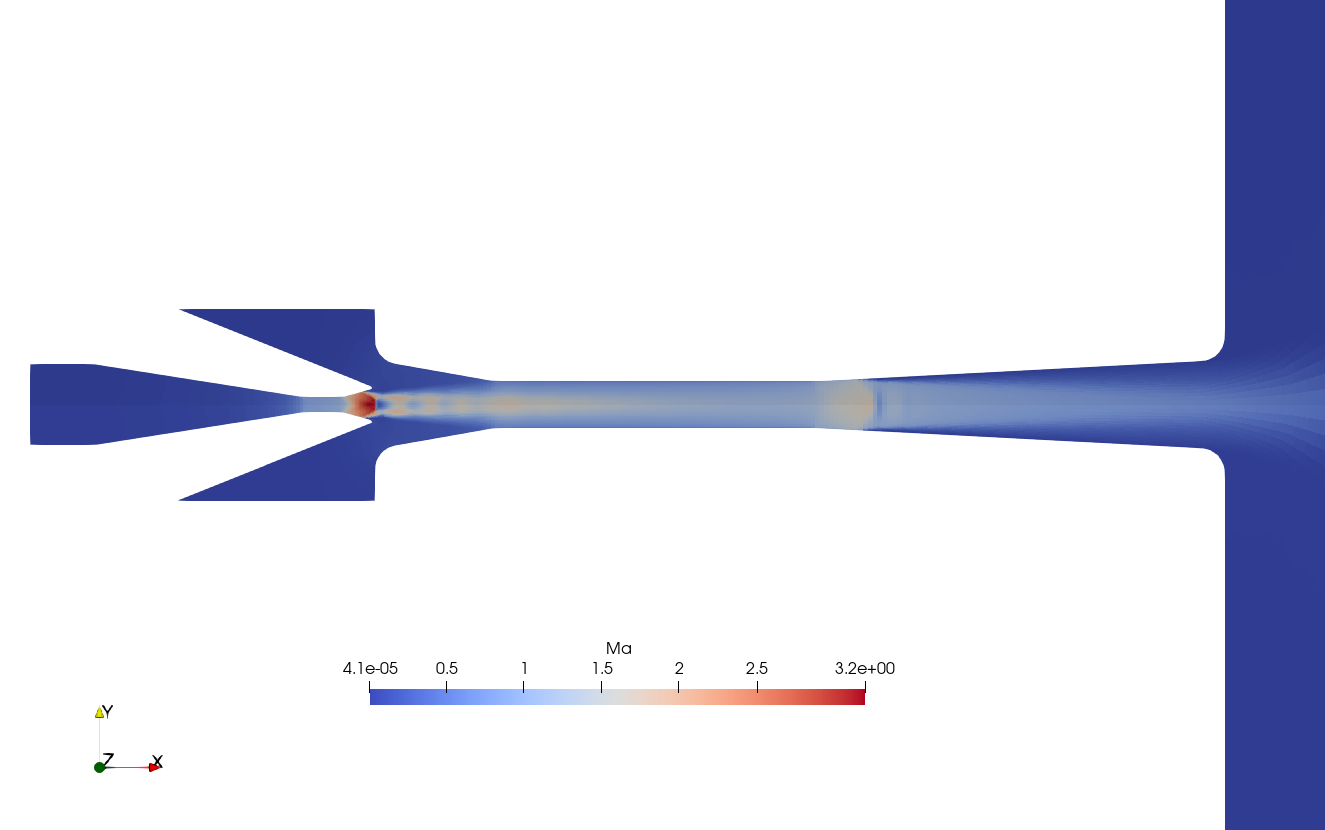
\includegraphics[width=\linewidth]{Figures/hisa_Ma}
	\caption{Mach number distribution}
	\label{fig:hisama}
\end{figure}


\section{Student Exercises and Extensions}

\subsection{Basic exercises for Part A: VOF}


\subsection{Basic exercises for Part B: Euler-Euler}



% ========== DISCLAIMER ============

\section*{Disclaimer}

This tutorial has been developed by \textbf{Robert Castilla}, 
of the Departament of Fluid
Mechanics in the Universitat Politècnica de Catalunya, for the doctoral 
workshop at \textbf{IMP⁻PAN Gda\'{n}sk} (July 2026). The author utilized \textbf{DeepSeek} for the initial
definition of the document format. Further technical refinement and the development
of advanced post-processing exercises were supported by \textbf{NotebookLM}. All the technical
information for the \textbf{OpenFOAM v2512} environmnet and all physical interpretations were
performed and approved by the author. 

% ========== END DOCUMENT ==========
\end{document}